\documentclass[10pt, openany]{book}

\usepackage{fancyhdr}
\usepackage{imakeidx}

\usepackage{amsmath}
\usepackage{amsfonts}

\usepackage{geometry}
\geometry{letterpaper}

\usepackage{fancyvrb}
\usepackage{fancybox}

\usepackage{url}
\usepackage{gensymb}
\usepackage{multicol}
\usepackage{tabularx}
%
% Rules to allow import of graphics files in EPS format
%
\usepackage{graphicx}
\DeclareGraphicsExtensions{.eps}
\DeclareGraphicsRule{.eps}{eps}{.eps}{}
%
% Macro definitions
%
\newcommand{\switch}[2]{``#1''/``#2''}
\newcommand{\position}[1]{``#1''}
%
% Front Matter
%
\title{General Purpose Discrete I/O Board}
\author{Brent Seidel \\ Phoenix, AZ}
\date{ \today }
%========================================================
%%% BEGIN DOCUMENT
\begin{document}
%
% Produce the front matter
%
\frontmatter
\maketitle
\begin{center}
This document is \copyright 2021 Brent Seidel.  All rights reserved.

\paragraph{}Note that this is a draft version and not the final version for publication.
\end{center}
\tableofcontents
\listoffigures
\listoftables

\mainmatter
%----------------------------------------------------------
\chapter{Introduction}
This circuit grew out of the Pi-Mainframe project.  It used two copies of this basic circuit to interface with a bunch of switches and LEDs.

This project replaces figure \ref{fig:Old-GPIO} with figure \ref{fig:New-GPIO}.  It should be obvious that the new style with the custom PCB will be easier to assemble.  The new PCB also has space for series resistors on all of the GPIOs.  This would allow a single PCB to drive 32 LEDs, or could be used to incorporate some input protection for switches.

\begin{figure}[ht!]
  \centering
  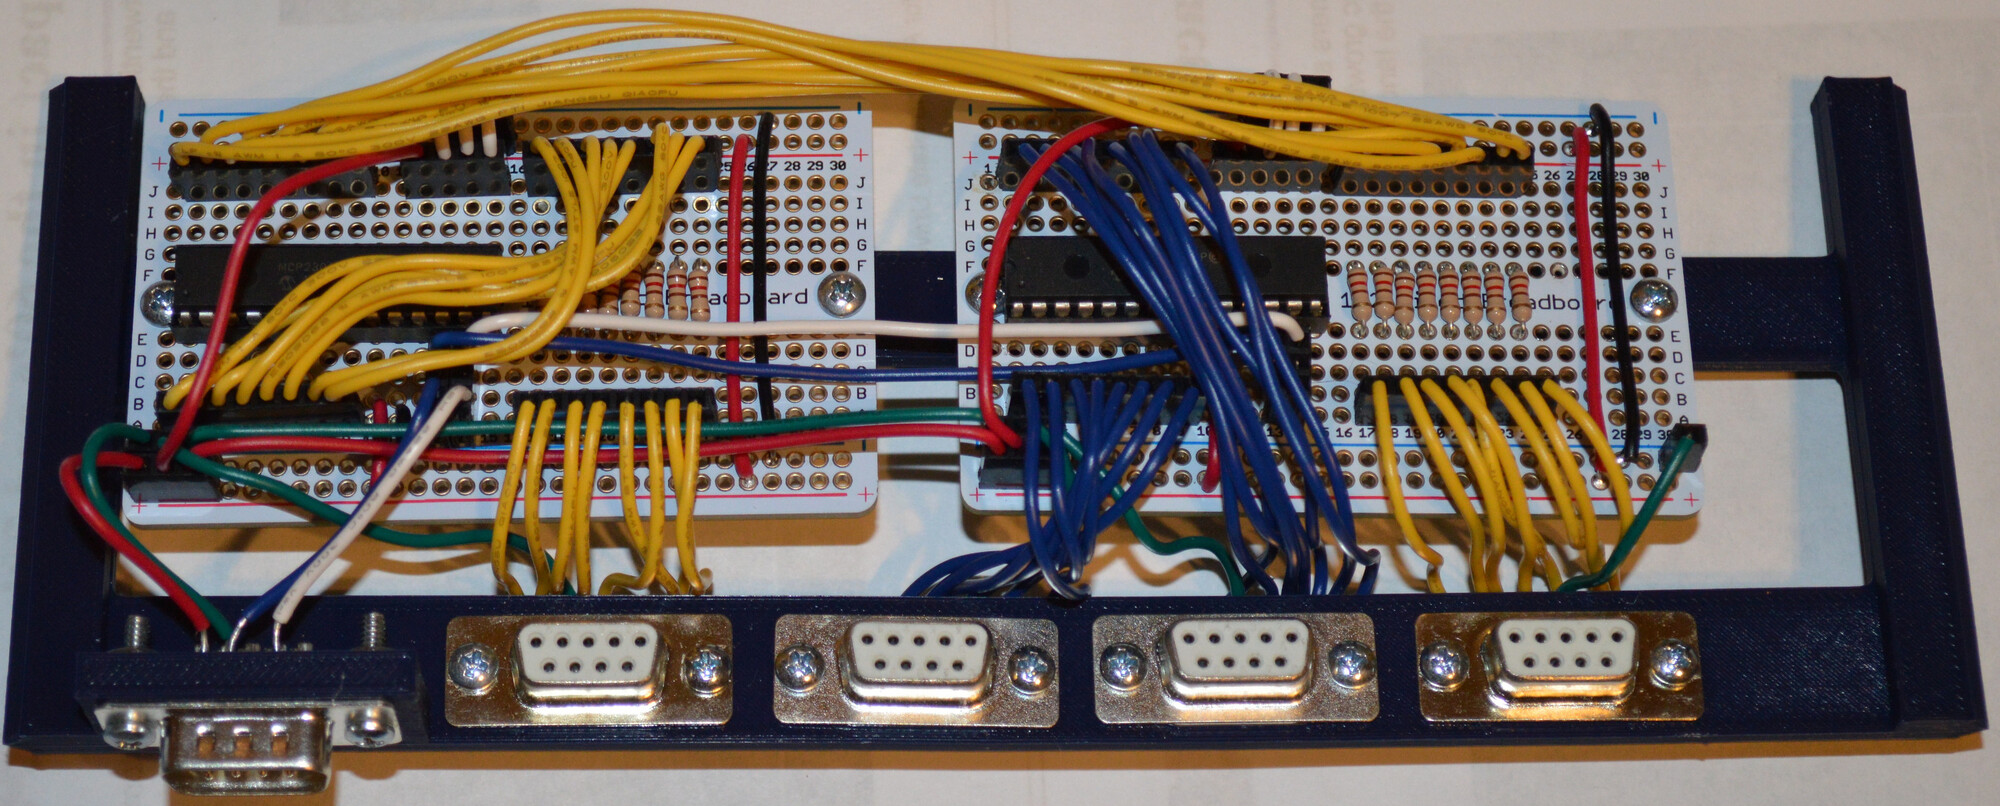
\includegraphics[width=0.9\textwidth]{../Pictures/Old Style.jpg}
  \caption{Old Style GPIO}
  \label{fig:Old-GPIO}
\end{figure}

\begin{figure}[ht!]
  \centering
  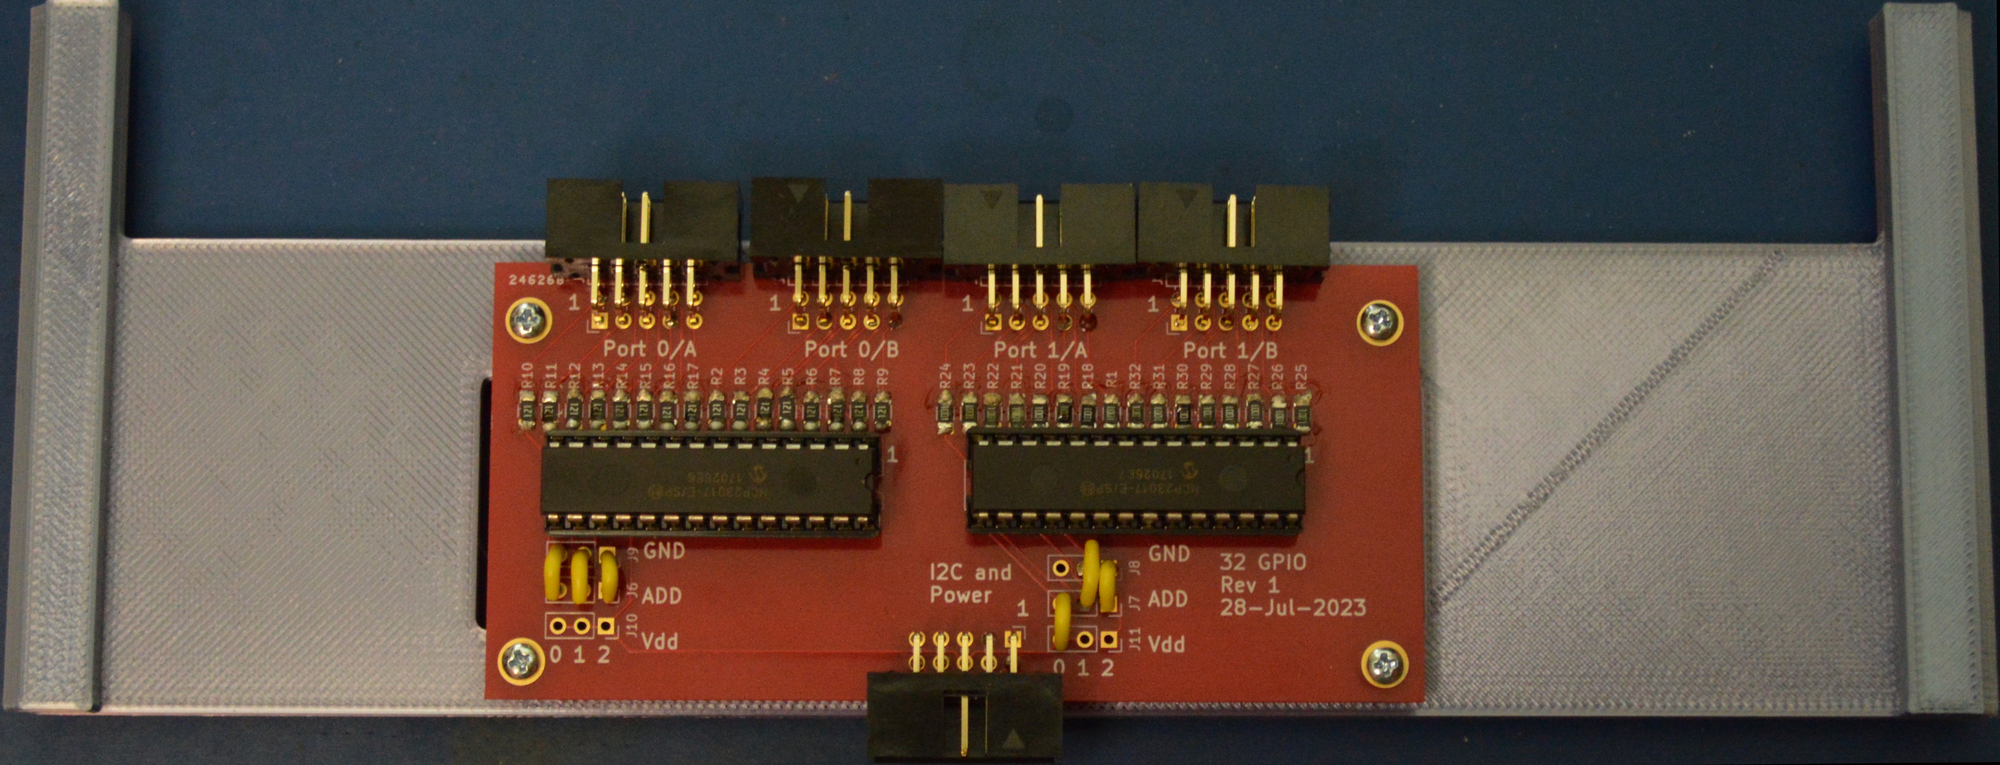
\includegraphics[width=0.9\textwidth]{../Pictures/Mounted.jpg}
  \caption{New GPIO PCB}
  \label{fig:New-GPIO}
\end{figure}


\section{Parts}
\subsection{Electronic Parts}
Note that this project requires soldering, but not as much as the old style.  It does however require soldering of SMD resistors.  These are a little finicky, but once you're got the method they don't take any longer than the through-hole resistors.

A public list of parts is available at DigiKey at \url{https://www.digikey.com/en/mylists/list/A5PCLNSPHC}.  I have also ordered the PCBs through DigiKey's PCB Builder tool and selected options to enable the DigiKey Red option which is cheaper.  Oddly, for a brief period, DigiKey allowed one to upload the KiCAD PCB file, but now it wants a zipped archive of the gerber files.  So, to get your PCBs, you will need to open KiCAD and export the gerber files (including the drill file) and archive them into a zip file.  Then upload it to the DigiKey.  If you already have a PCB place you use, you probably already know what to do for them.

The other parts required are (all parts are through-hole, except for the SMD resistors:
\begin{itemize}
  \item 32 SMD 1206 size resistors.  I use $120\Omega$ for the LED and 1K for the switches.  Select whatever you need for your application.  When ordering, look for price breaks for bulk pricing.  I ordered 500 of each.
  \item 2 MCP23017 ICs.
  \item 2 28 pin sockets 0.3 width.  These are optional, but I like to use sockets for my ICs.
  \item 5 right angle 10 position (2x5) connectors.
  \item 6 short pieces of jumper wire for setting the device addresses.
\end{itemize}

%----------------------------------------------------------
\chapter{Hardware}

\subsection{Planning}
The two main things that need to be decided before assembling the board are the resistor values for your application.  If you are using a 3.3V powered CPU (such as a Raspberry PI) and driving LEDs, $120\Omega$ resistors should work, but they may be on the low end.  If you are using a 5V powered CPU (such as some Arduinos), you would need a slightly higher value.  There is actually a fairly broad range of values that work.  The next thing to be decided is the I2C addresses for each chip.  Giving multiple devices the same addresses on the same bus will only lead to sorrow, so it would be a good idea to plan out the addresses for all the devices (not just the I/O board) you are going to use on that bus.

\section{Assembly}
Make sure that you have a good soldering iron, solder, plenty of light.  You may also want a magnifier and some device to hold the board.  I like to start working with the shortest components first and work my way up to taller and taller components.

\subsection{SMD Resistors}
The first step is to solder the SMD resistors.  If you already have experience with soldering SMD devices, you can skip this.  If not, here is my wisdom gained from soldering precisely 64 SMD resistors as of this writing.

First put a small blob of solder on one of the SMD pads.  You can do this for multiple resistors in one step as shown in figure \ref{fig:SMD-1}.  The figure shows the resistors for port 0 all done.

\begin{figure}[ht!]
  \centering
  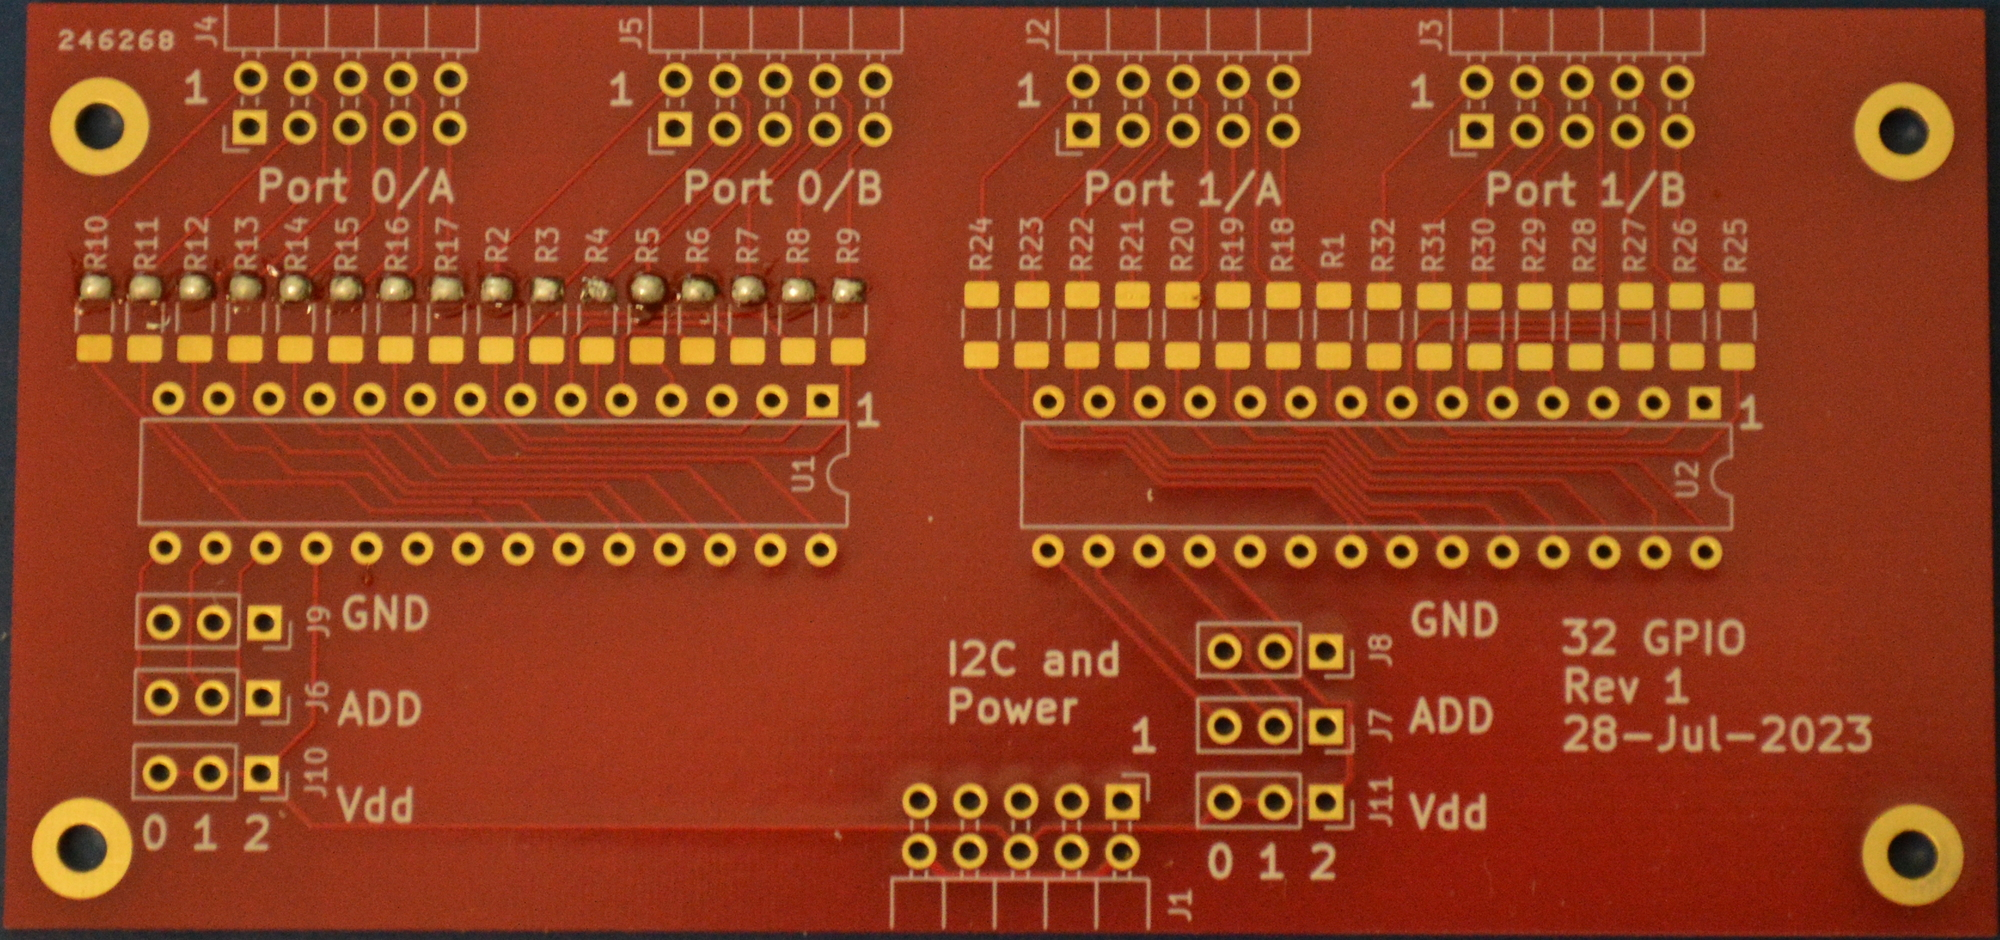
\includegraphics[width=0.9\textwidth]{../Pictures/SMD-1.jpg}
  \caption{Soldering SMD Resistors, Step 1}
  \label{fig:SMD-1}
\end{figure}

Next pick up a resistor with tweezers and move it to the solder blob while melting the blob with you soldering iron.  Be careful as the resistors have a tendency to make a mad dash for freedom while you are trying to move them.  Once one end is in the solder, remove the iron and let the solder harden.  This secures the resistor in place for soldering the other end.  Figure \ref{fig:SMD-2} shows the resistors for port 0 all with one end soldered.

\begin{figure}[ht!]
  \centering
  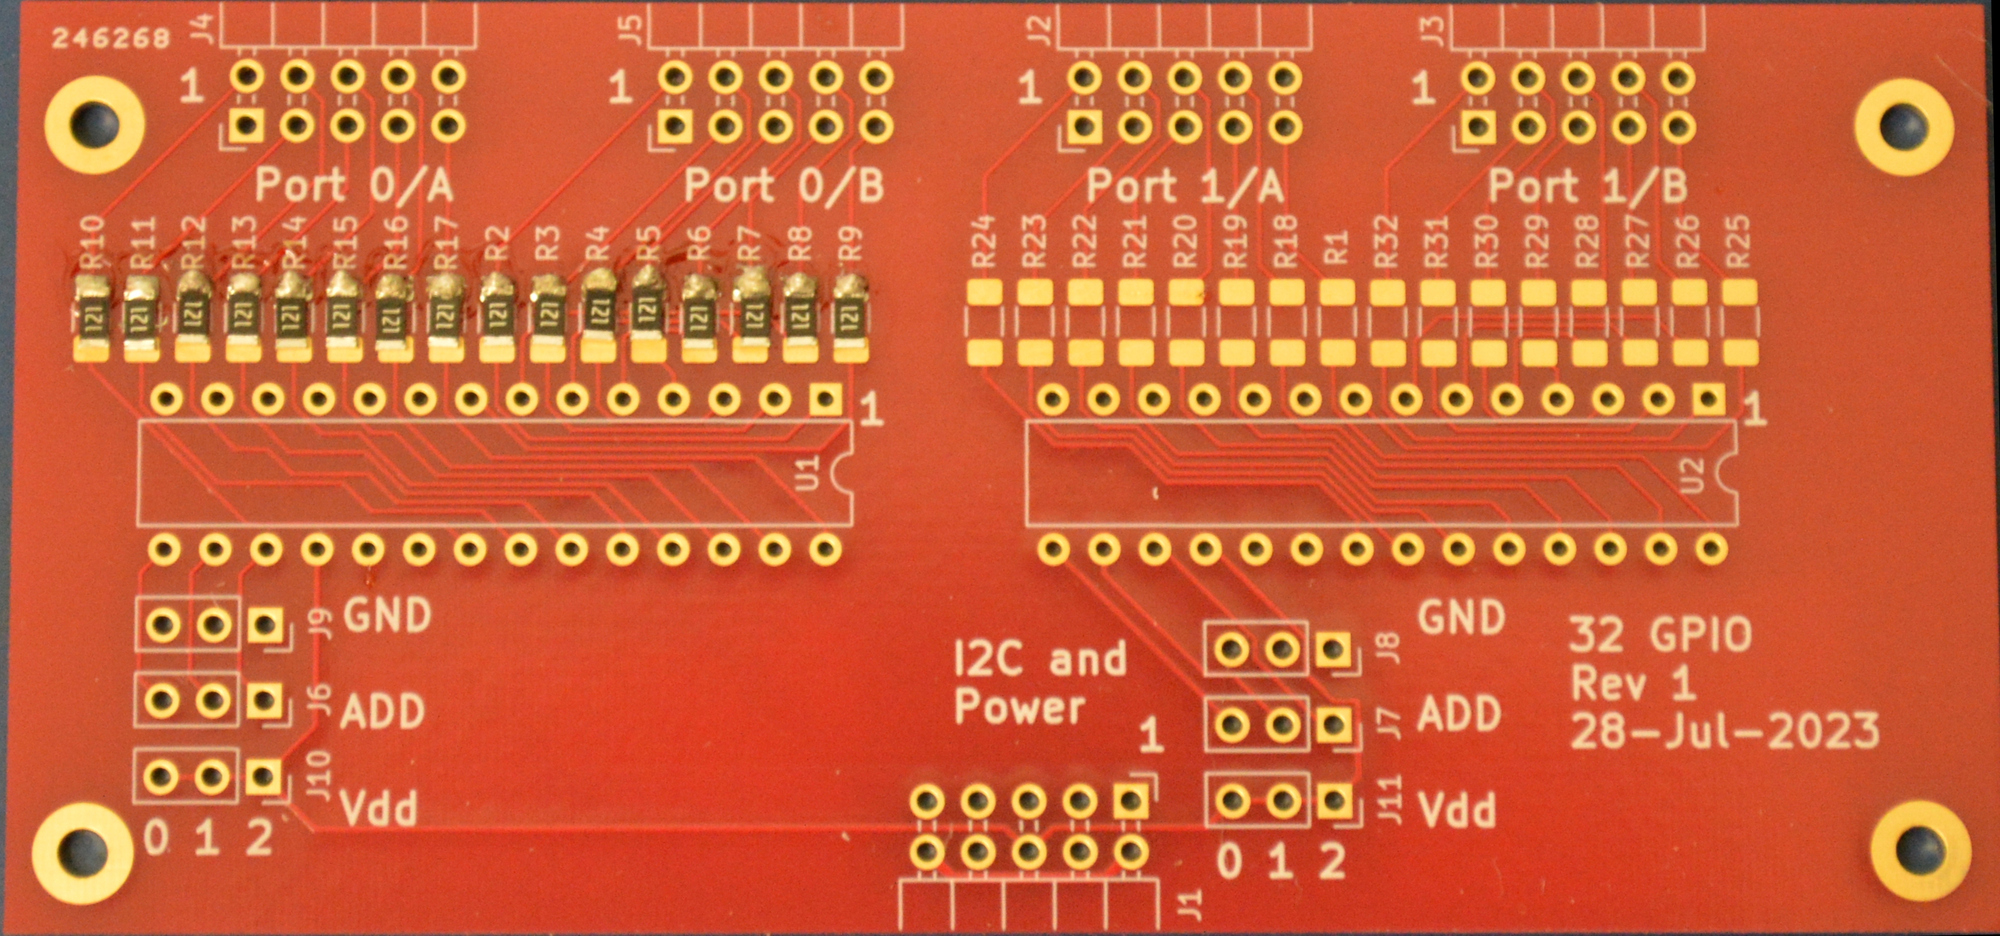
\includegraphics[width=0.9\textwidth]{../Pictures/SMD-2.jpg}
  \caption{Soldering SMD Resistors, Step 2}
  \label{fig:SMD-2}
\end{figure}

Finally solder the other end of each resistor (figure \ref{fig:SMD-3}) and finish up the rest of the resistors (figure \ref{fig:SMD-4}).

\begin{figure}[ht!]
  \centering
  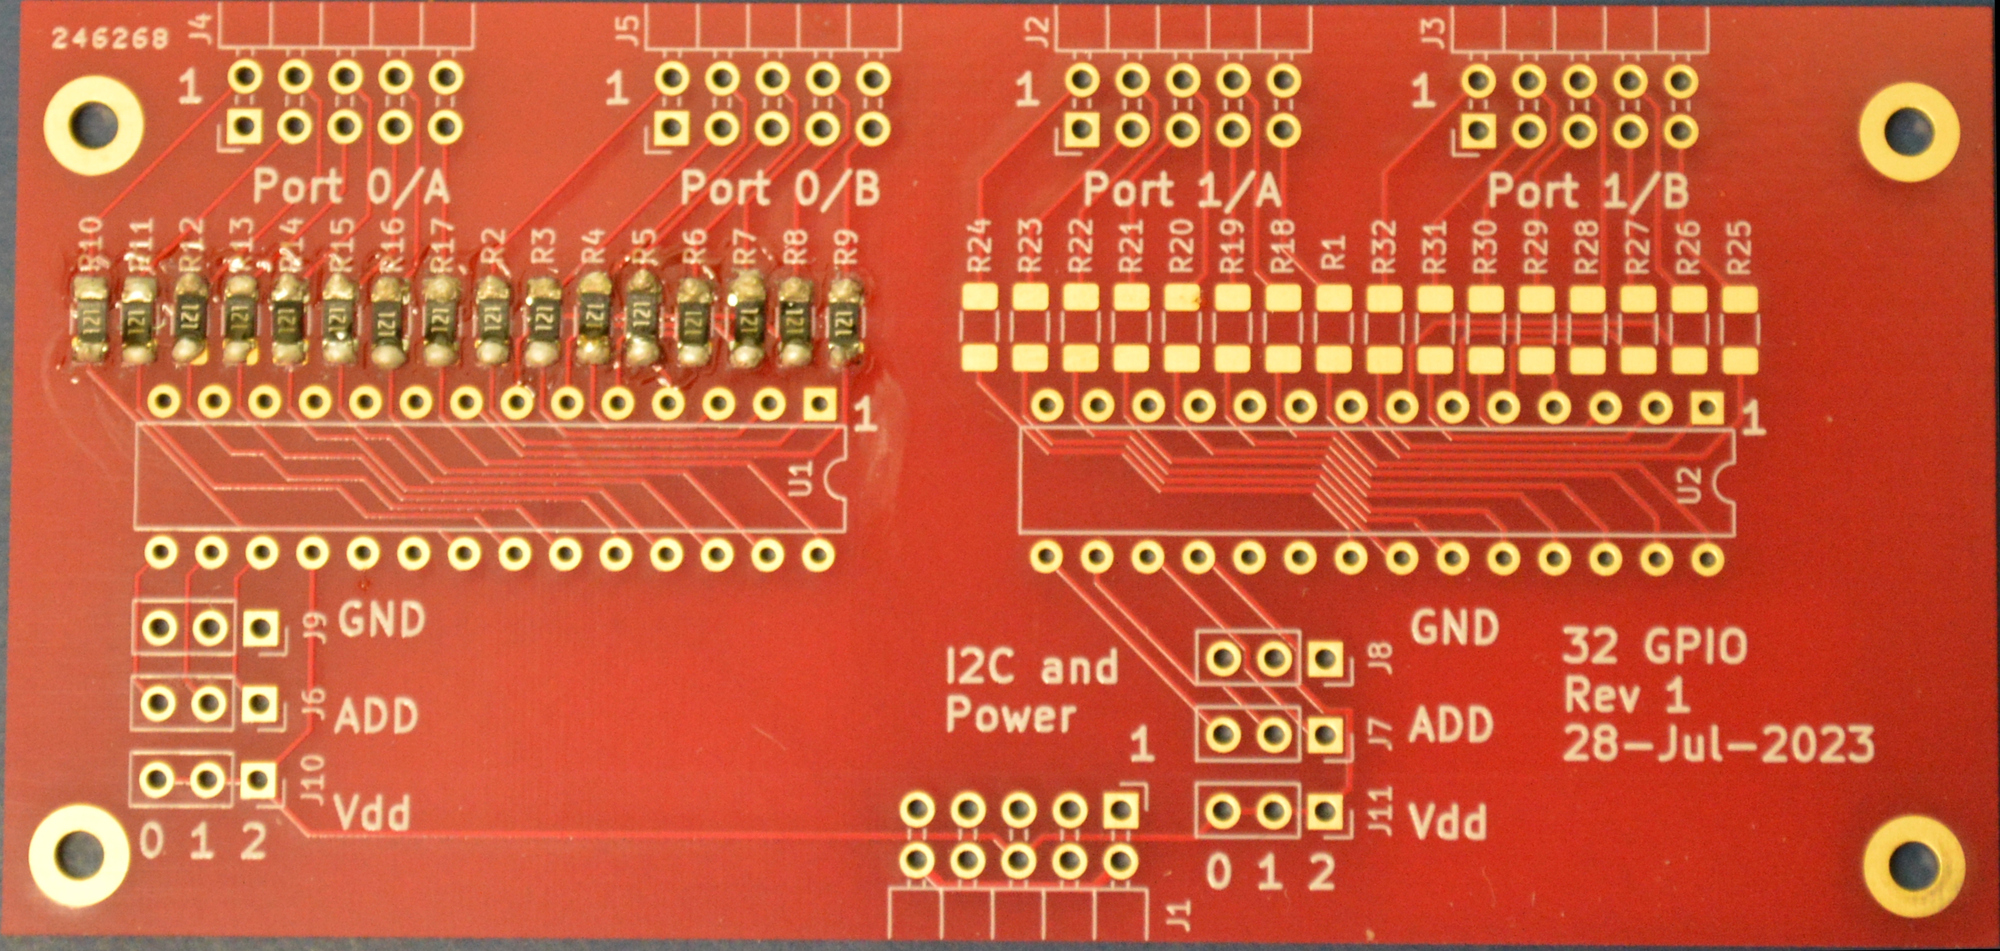
\includegraphics[width=0.9\textwidth]{../Pictures/SMD-3.jpg}
  \caption{Soldering SMD Resistors, Step 3}
  \label{fig:SMD-3}
\end{figure}

\begin{figure}[ht!]
  \centering
  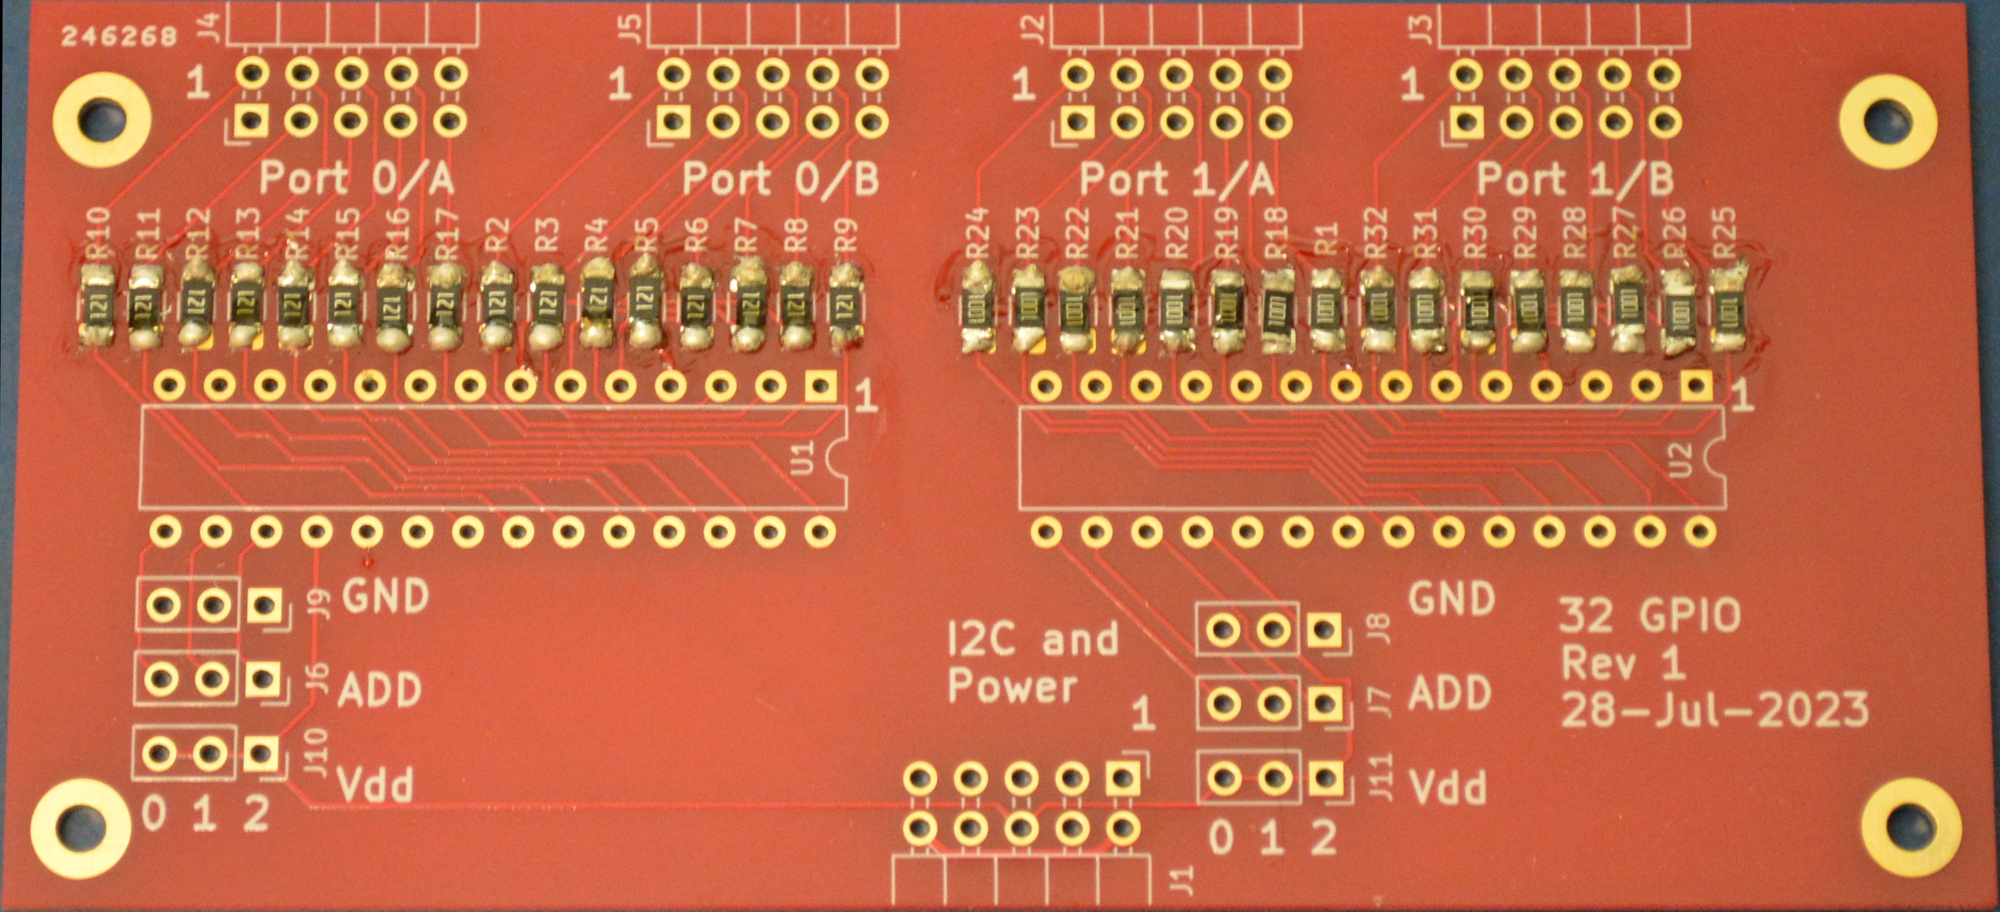
\includegraphics[width=0.9\textwidth]{../Pictures/SMD-4.jpg}
  \caption{Soldering SMD Resistors, Step 4}
  \label{fig:SMD-4}
\end{figure}

\clearpage
\subsection{Other Components}
The rest of the components are fairly conventional.  The only issue that I encountered is that I had ordered the 0.600 width IC sockets instead of 0.300 width.  If you have the correct size or are not using sockets, you can ignore this bit.  If you need to hack your sockets, this may be interesting.  There were only a couple of strips of plastic connecting the two sides of the socket.  It was easy to cut them off with wire cutter, leaving me with 2 separate 14 pin strips.  To ensure that they were soldered in proper alignment, I put them on an IC, inserted them into the PCB and soldered them that way.  The end result is in figure \ref{fig:Sockets}.  This turned out OK, though if you look closely, you can see the missing connections between the two sides of the socket.  You can also see why you want to solder the SMD resistors first - there is not much room between the socket and the resistors.

\begin{figure}[ht!]
  \centering
  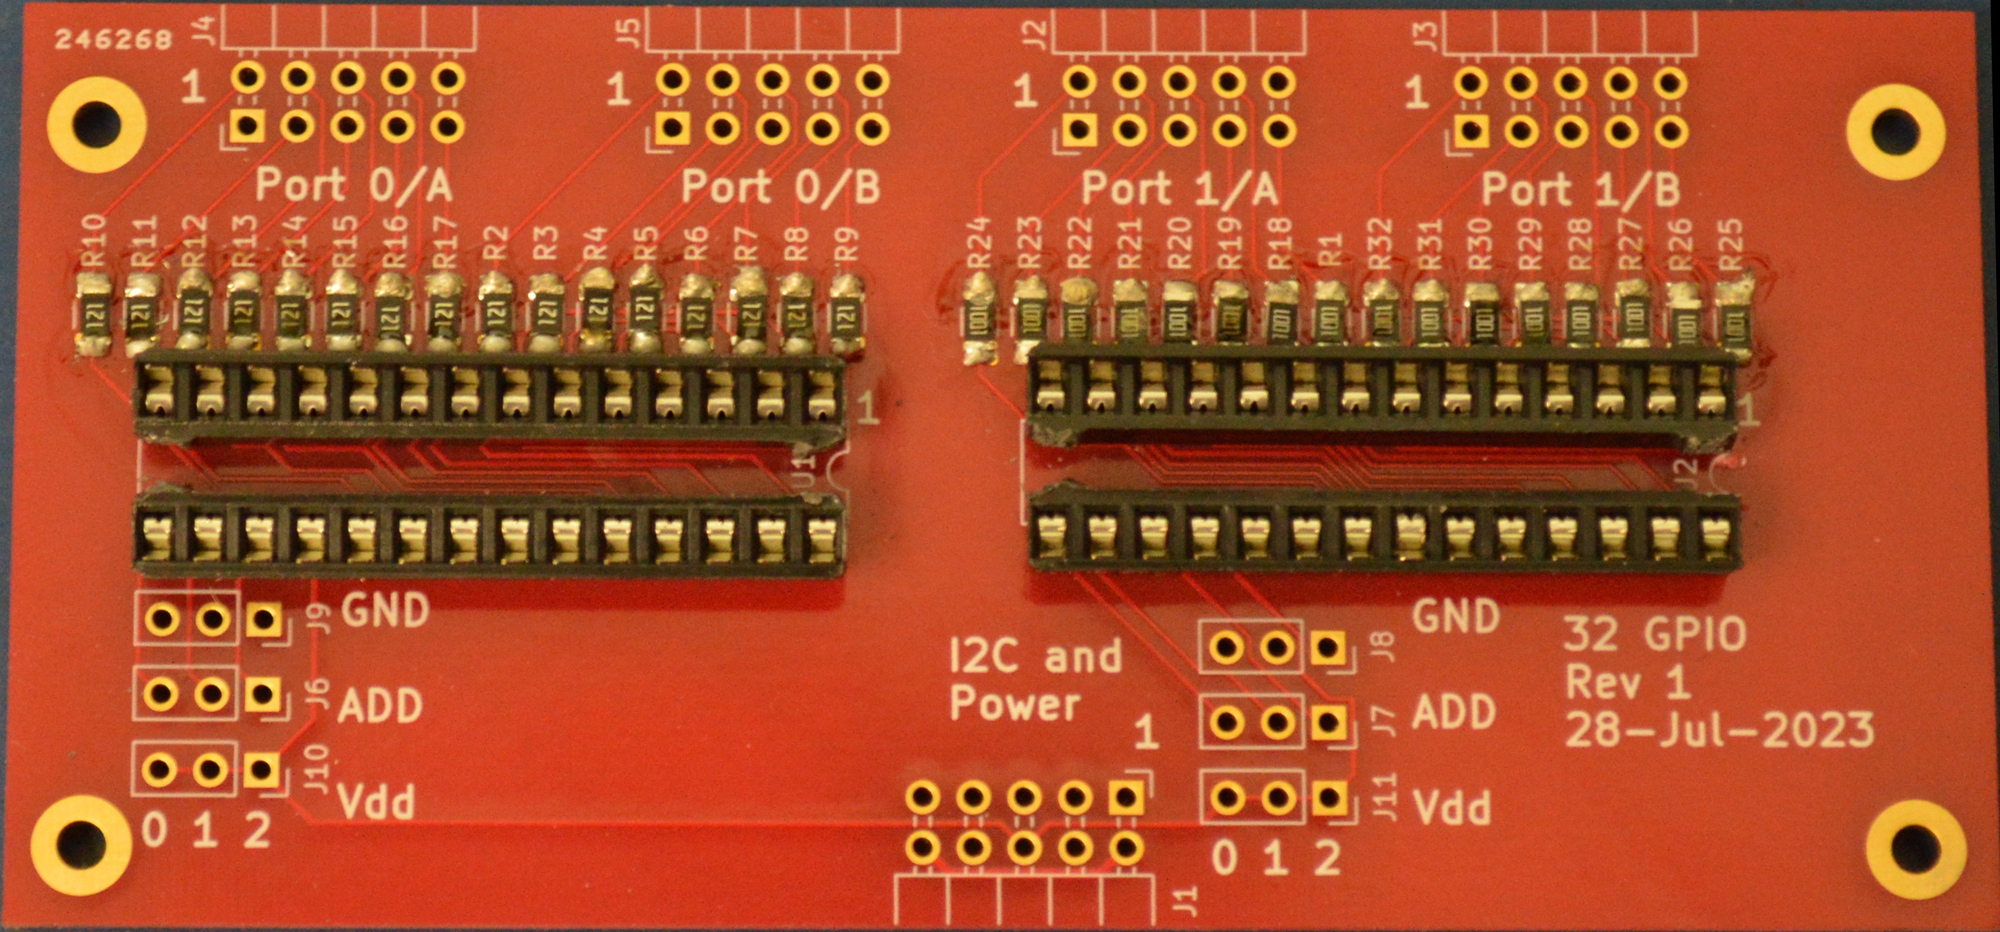
\includegraphics[width=0.9\textwidth]{../Pictures/Sockets.jpg}
  \caption{Soldering IC Sockets}
  \label{fig:Sockets}
\end{figure}

The connectors that I used have a plastic shell around them.  Some of the connections at the top of the board were almost too close together, but it all fit.  These are fairly conventional to solder.  Just insert the connector and solder the pins.  It helps to level the board if you do the bottom connector and a couple of the top connectors at the same time.  The end result should be something like figure \ref{fig:Connectors}.

\begin{figure}[ht!]
  \centering
  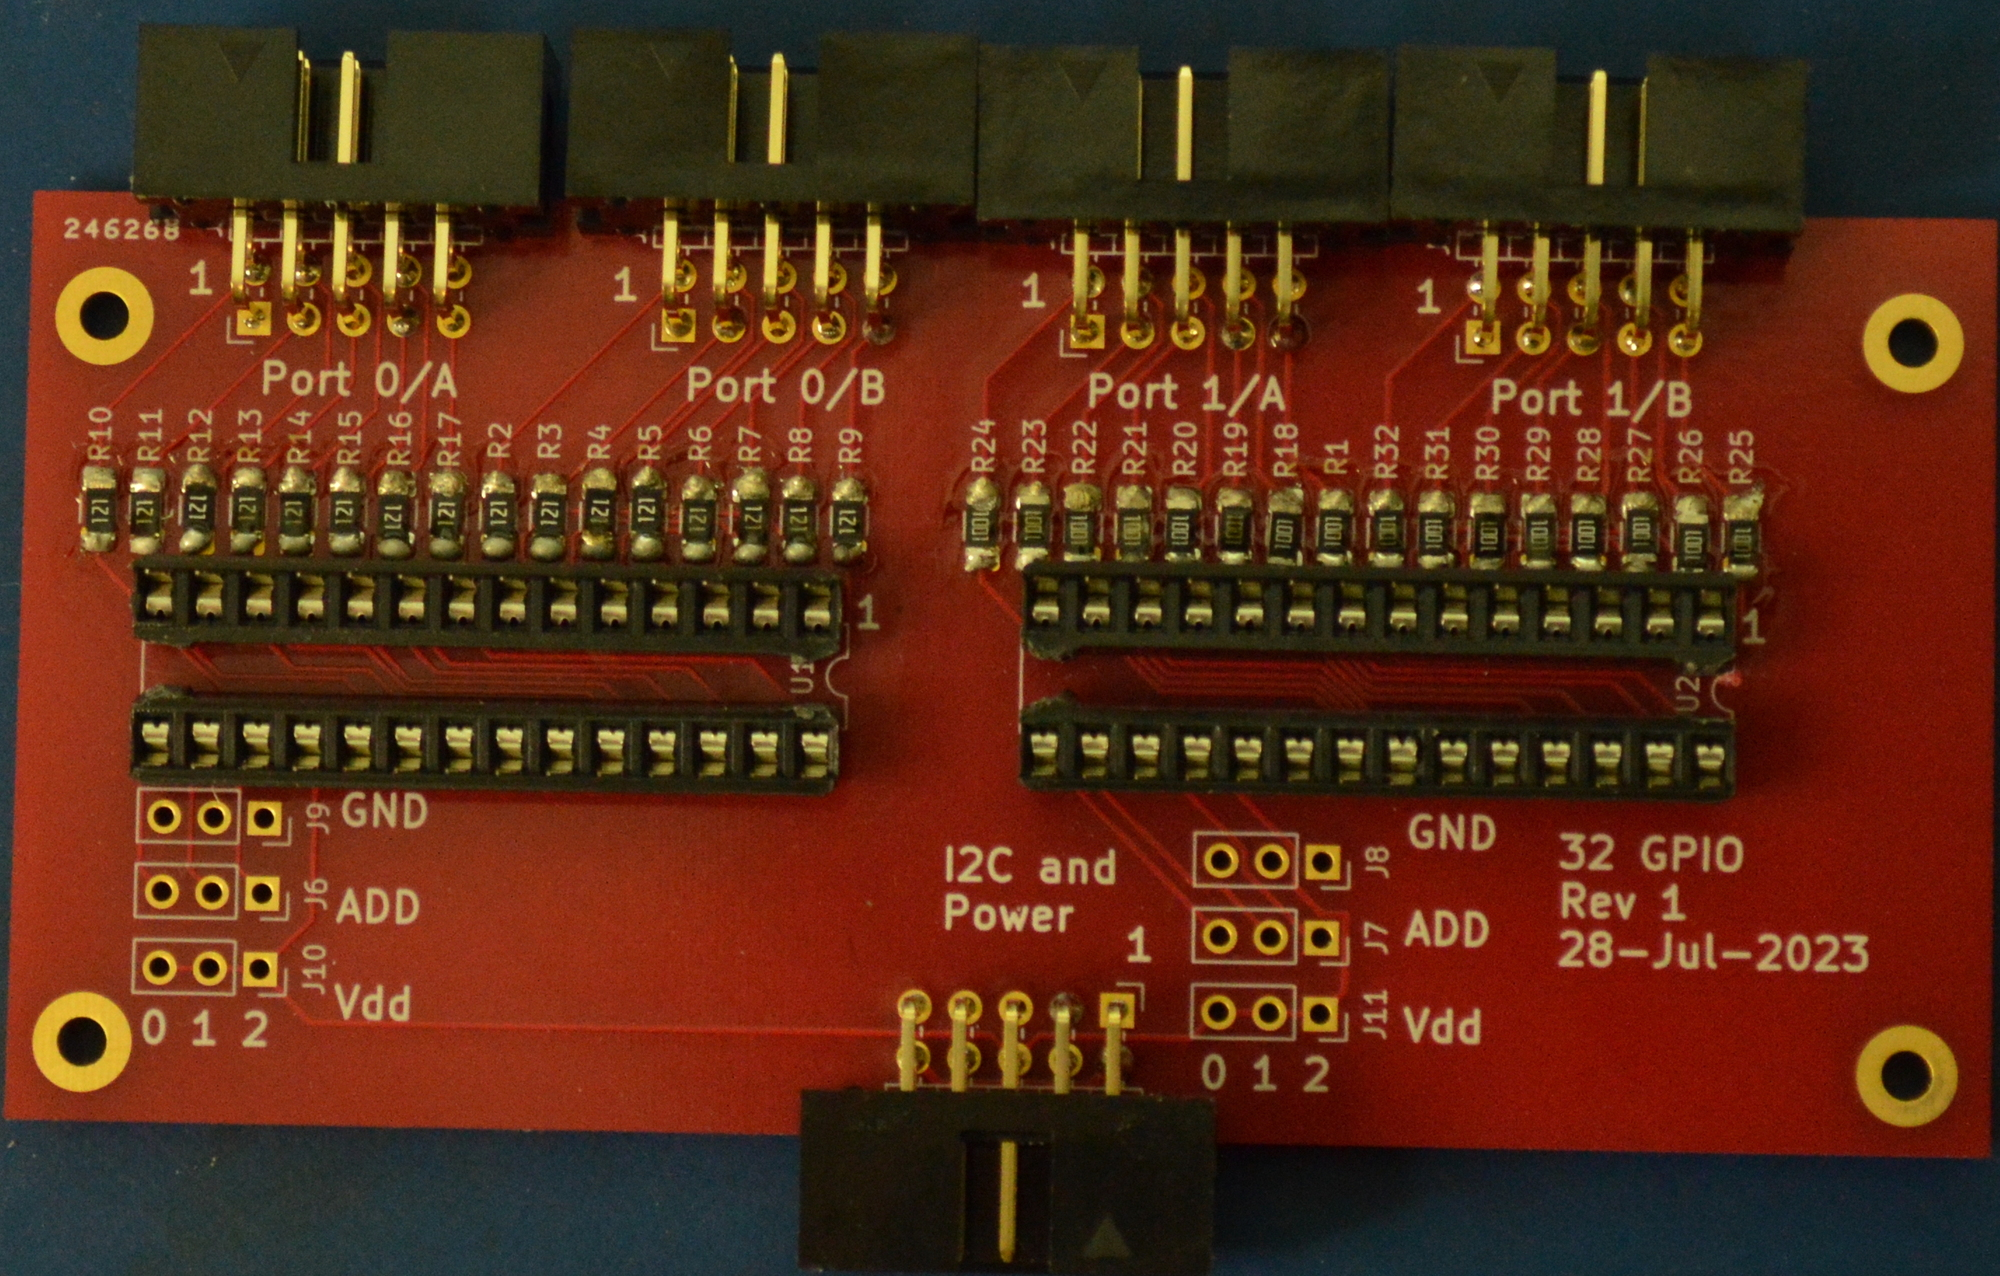
\includegraphics[width=0.9\textwidth]{../Pictures/Connectors.jpg}
  \caption{Board with Connectors Added}
  \label{fig:Connectors}
\end{figure}

Finally solder the jumpers to set the I2C address for each IC.  Three address bits are available giving 8 possible addresses.  Solder a jumper from ADD to GND for a 0 and from ADD to Vdd for a 1.  An example is in figure \ref{fig:Jumpers}.  This shows the IC on the left with an address of $20_{16}$ and the IC on the right with an address of $21_{16}$ (the $2x_{16}$ part is supplied by the IC.  The $x$ part is set by the jumpers to 0-7. If you need to change an address for some reason, it would be fairly easy to unsolder a jumper and move it.

\begin{figure}[ht!]
  \centering
  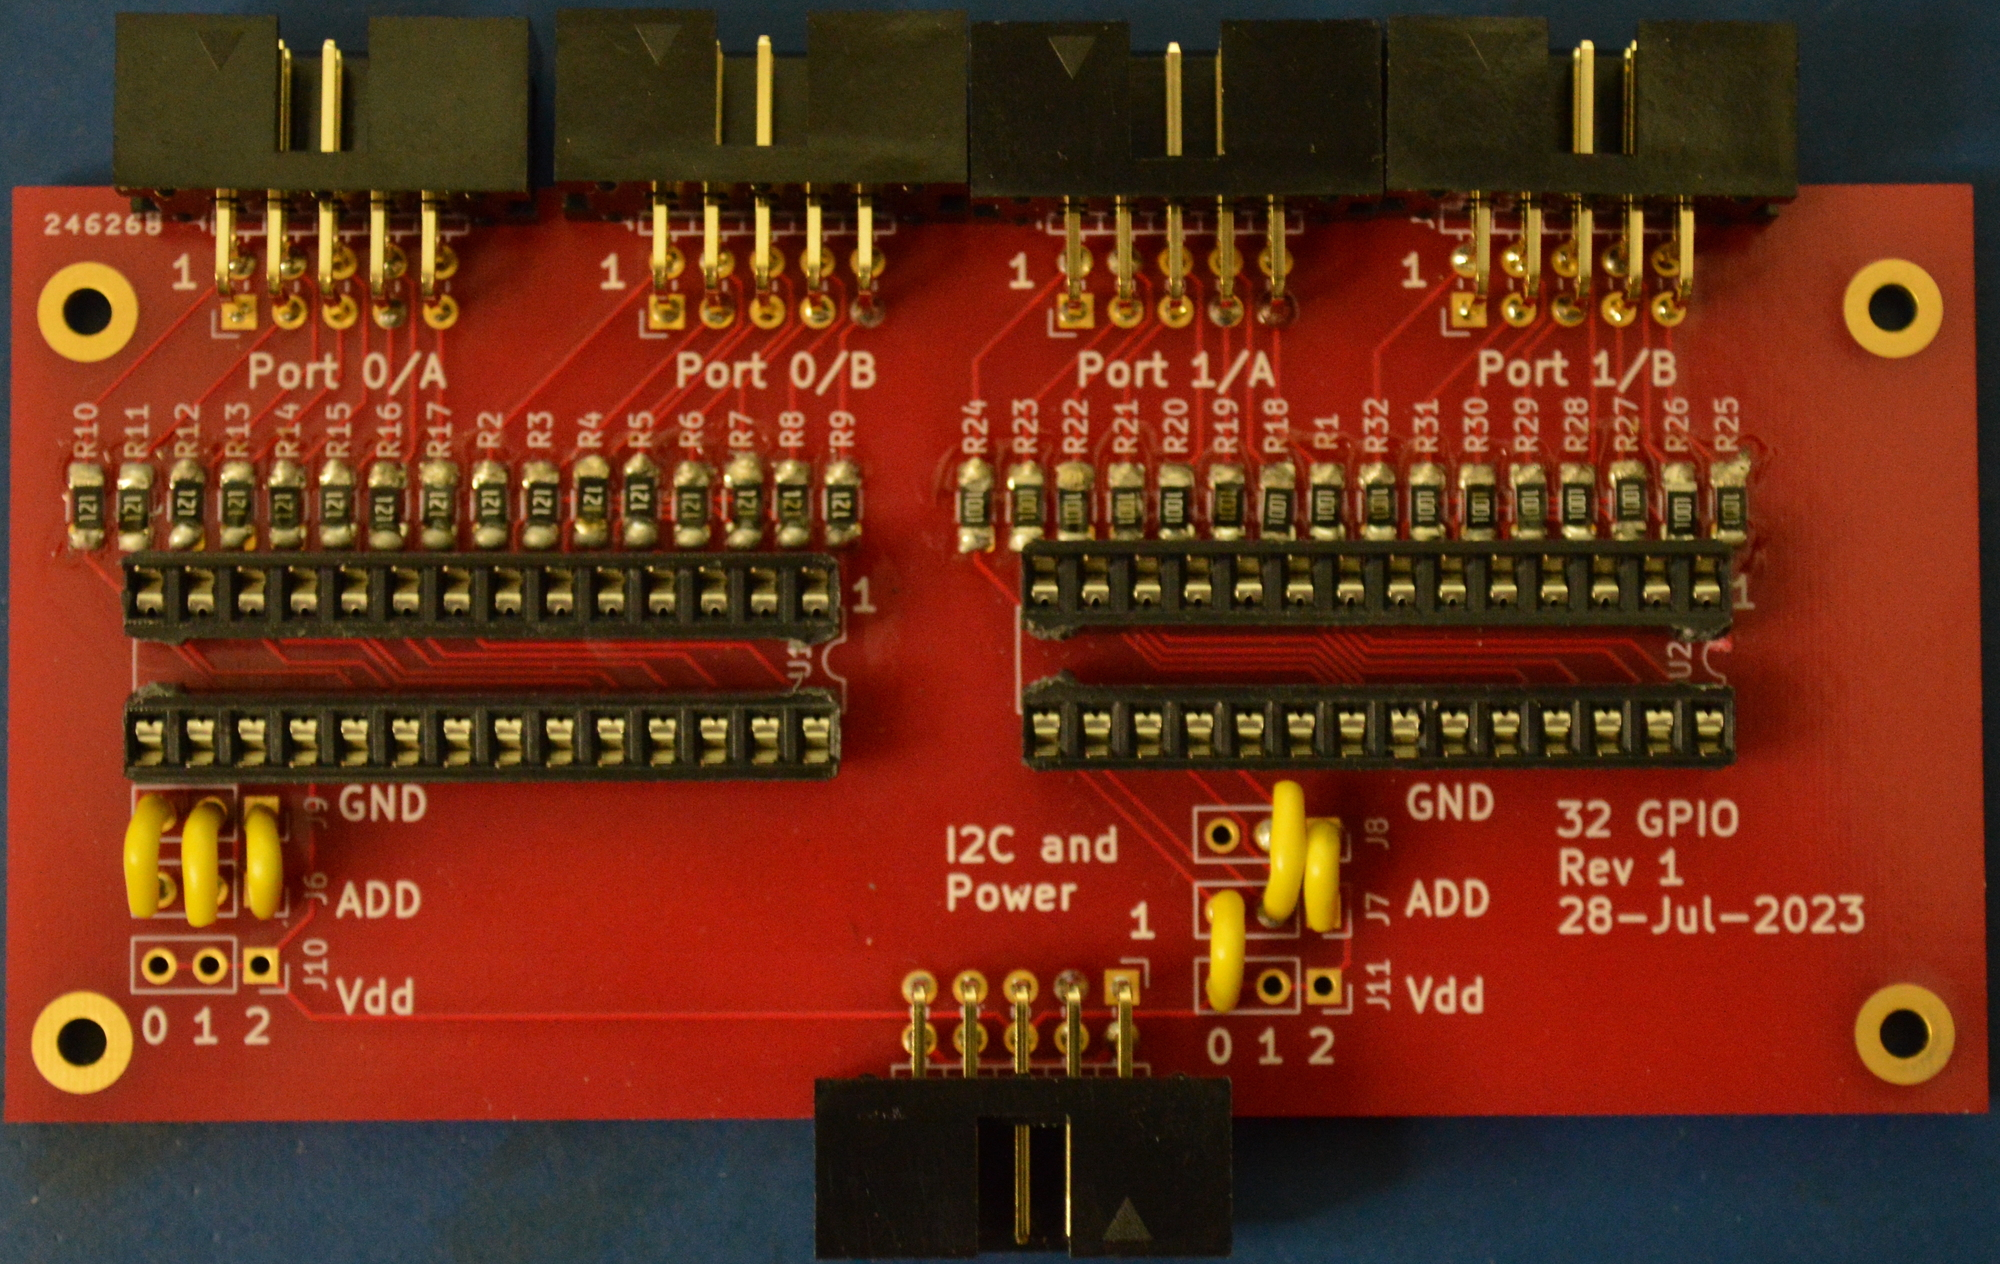
\includegraphics[width=0.9\textwidth]{../Pictures/Jumpers.jpg}
  \caption{Board with Address Jumpers Inserted}
  \label{fig:Jumpers}
\end{figure}

There are spaces on the back of the board where you can make notes for whatever you find useful.  An example is in figure \ref{fig:Notes} where I identify the resistor values and note that this is a board for testing.  It may be best to add the notes after you are finished with soldering.

\begin{figure}[ht!]
  \centering
  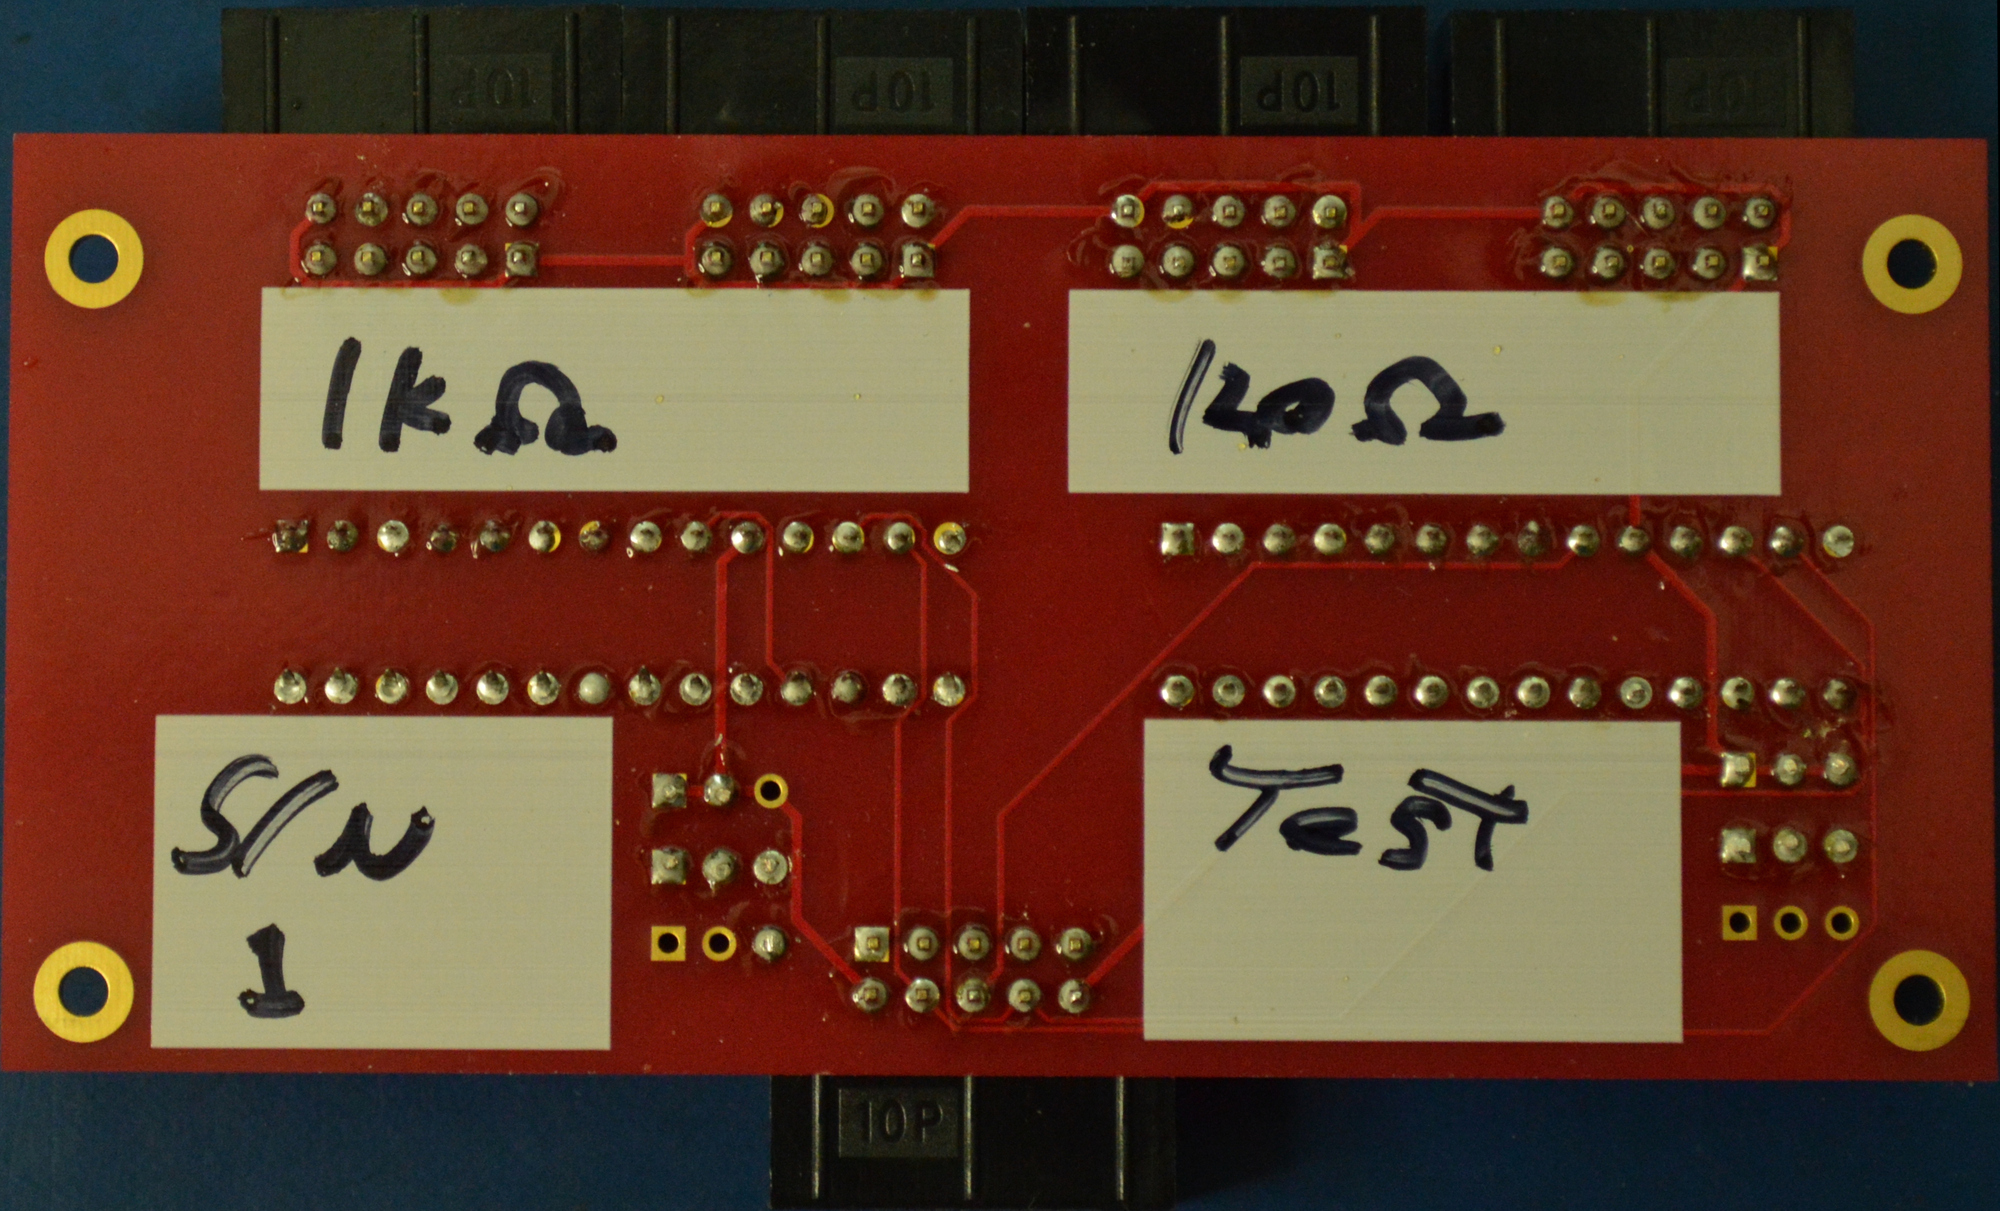
\includegraphics[width=0.9\textwidth]{../Pictures/Notes.jpg}
  \caption{Back of Board with Notes}
  \label{fig:Notes}
\end{figure}

Finally, insert the ICs and the board is done.  If you soldered the ICs directly to the board, then you are already done.  The top of the finished board should look something like figure \ref{fig:Complete}.

\begin{figure}[ht!]
  \centering
  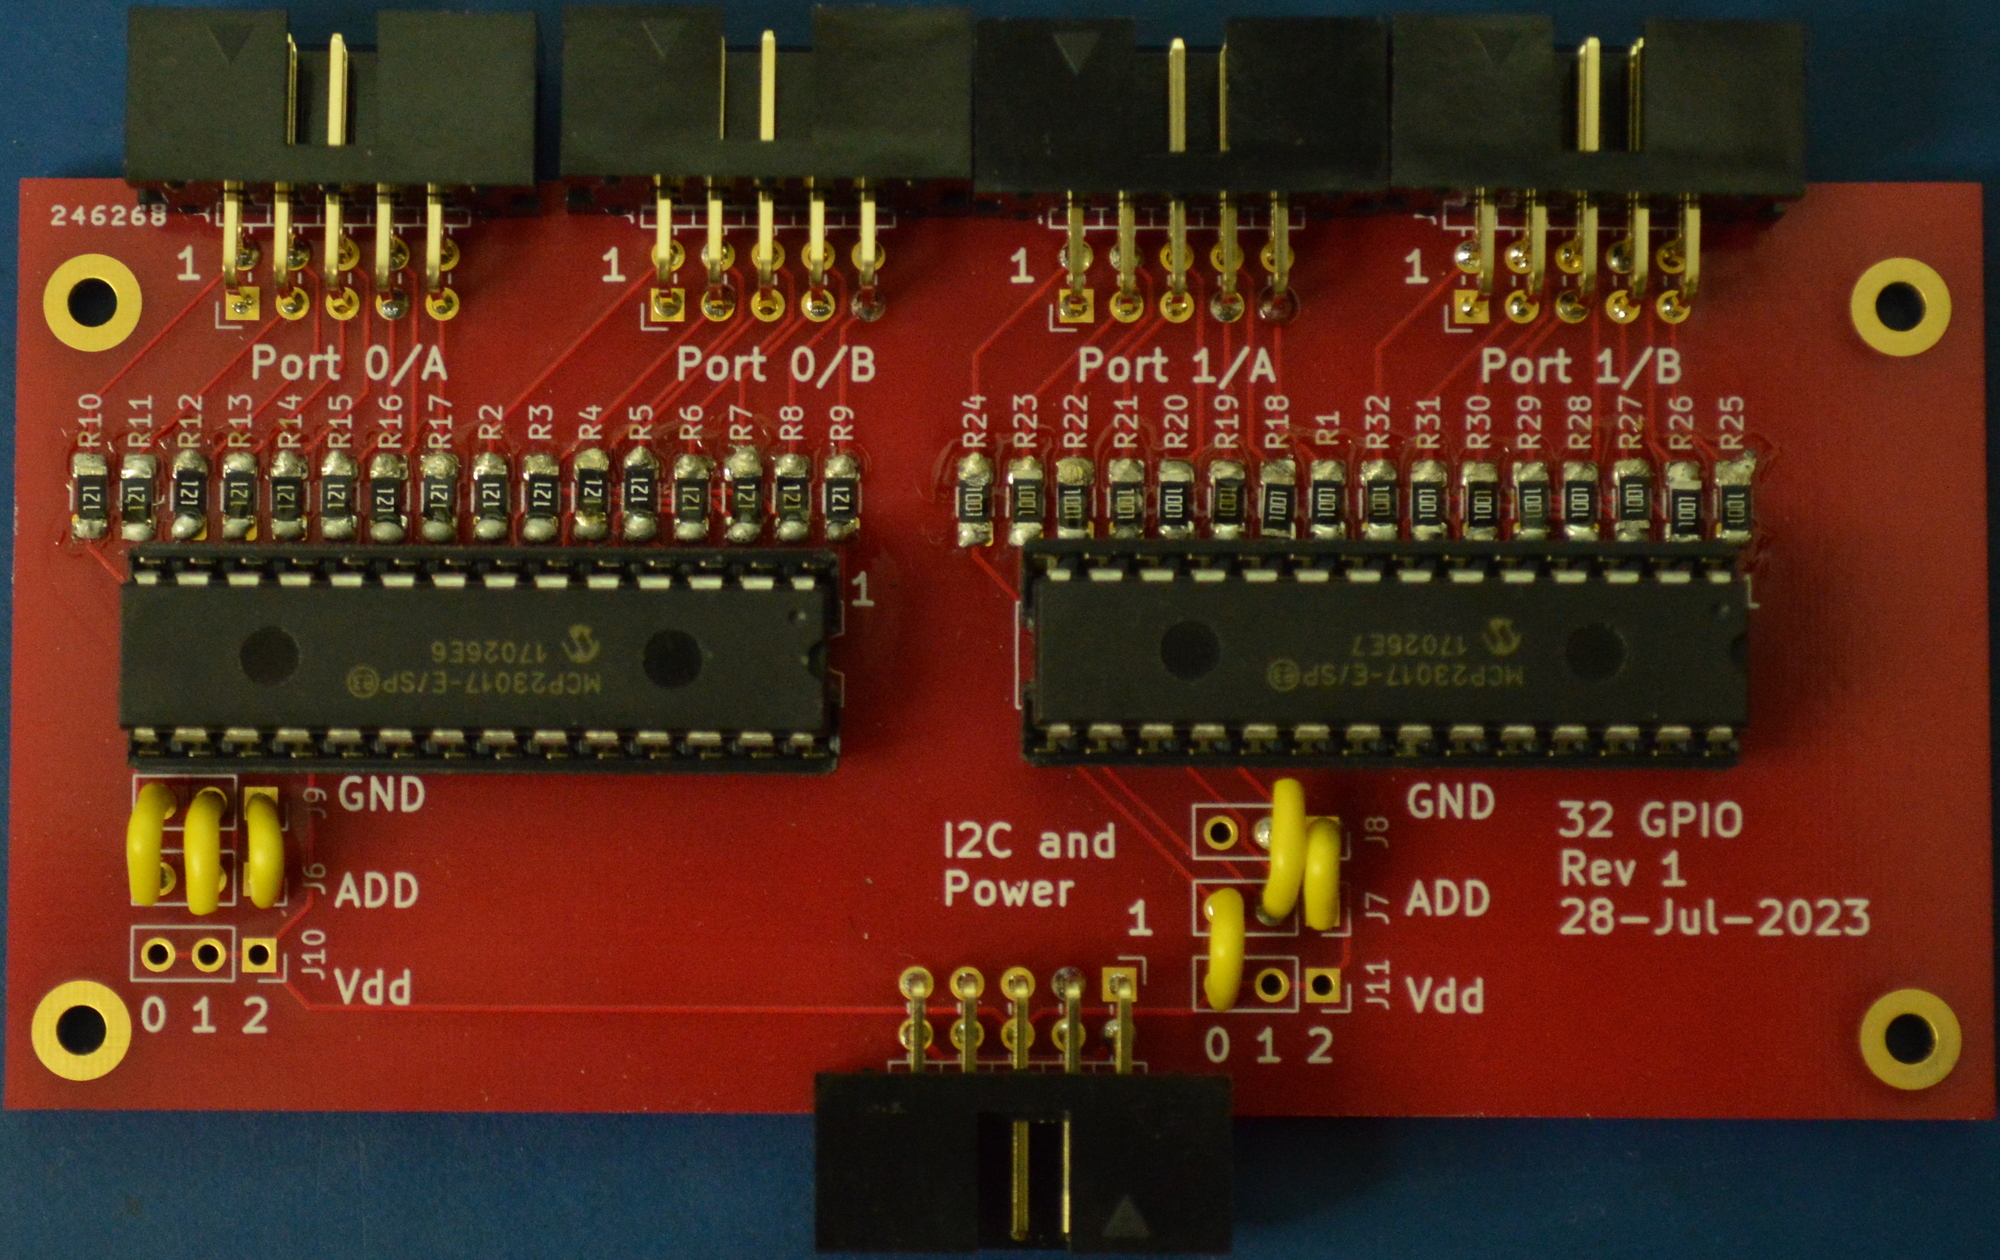
\includegraphics[width=0.9\textwidth]{../Pictures/ICs.jpg}
  \caption{Completed Board}
  \label{fig:Complete}
\end{figure}

\clearpage
\subsection{GPIO Connector Pinouts}
The connectors pins are in odd-even format with pin 1 being identify by a square solder pad.  This row is odd numbered (1-3-5-7-9).  The other row is even numbered (2-4-6-8-10).  The pins are as identified in table \ref{tbl:GPIO-Pins} for each port.

\begin{table}
  \label{tbl:GPIO-Pins}
  \caption{GPIO Connector Pinout}
  \centering
  \begin{tabular}{|r|l|}
    \hline
    Pin & Description\\
    \hline
    1 & Ground\\
    2 & GPIO Pin 0\\
    3 & GPIO Pin 1\\
    4 & GPIO Pin 2\\
    5 & GPIO Pin 3\\
    6 & GPIO Pin 4\\
    7 & GPIO Pin 5\\
    8 & GPIO Pin 6\\
    9 & GPIO Pin 7\\
    10 & Ground\\
    \hline
  \end{tabular}
\end{table}

\subsection{I2C Connector Pinout}
The connectors pins are in odd-even format with pin 1 being identify by a square solder pad.  This row is odd numbered (1-3-5-7-9).  The other row is even numbered (2-4-6-8-10).  The pins are as identified in table \ref{tbl:I2C-Pins}.  Note that the odd row is not used by this board and all the odd numbered pins are no connection.  They may be used for other applications.  Leaving these as unused means that if the connector is inserted backwards, no pins will be connected, thus providing some protection against improperly powering IC pins.

\begin{table}
  \label{tbl:I2C-Pins}
  \caption{I2C Connectior Pinout}
  \centering
  \begin{tabular}{|r|l|}
    \hline
    Pin & Description\\
    \hline
    1 & No Connection\\
    2 & Ground\\
    3 & No Connection\\
    4 & SDA\\
    5 & No Connection\\
    6 & Vdd\\
    7 & No Connection\\
    8 & SCK\\
    9 & No Connection\\
    10 & Ground\\
    \hline
  \end{tabular}
\end{table}

%----------------------------------------------------------
\chapter{Programming}
For definitive information, refer to the MCP23017 data sheet.  This describes both the software and electrical interfaces to the ICs.  Each IC provides 16 GPIO pins.  These can be treated as one 16 bit port or two 8 bit ports.  Each pin can be configured to be an input or an output.  A weak pull-up can also be configured for inputs.

For Ada programming, a set of routines for interfacing to the MCP23017 are in the \url{https://github.com/BrentSeidel/BBS-BBB-Ada.git} repository.  Adafruit has an interface using CircuitPython with more information at \url{https://learn.adafruit.com/using-mcp23008-mcp23017-with-circuitpython/overview}.  An Arduino library is at \url{https://github.com/adafruit/Adafruit-MCP23017-Arduino-Library.git}.  Of course, an example of use and programming is in the original repository for this circuit, \url{https://github.com/BrentSeidel/Pi-Mainframe.git}.
\end{document}

